%Thanks to joseleite19, Tiagosf00, brunomaletta and naim-santos notebooks.
\documentclass{article}

\usepackage[utf8]{inputenc}
\usepackage[T1]{fontenc}
\usepackage{multicol}
\usepackage{listings}
\usepackage{xcolor}
\usepackage{graphicx}

%\usepackage[top=2cm, bottom=1.5cm, left=1cm, right=1cm]{geometry} 
\usepackage[landscape, left=0.5cm, right=0.5cm, top=1cm, bottom=1.5cm]{geometry} %pra deixar a margem do jeito que o brasil gosta

\definecolor{codegreen}{rgb}{0,0.6,0}
\definecolor{codegray}{rgb}{0.5,0.5,0.5}
\definecolor{codepurple}{rgb}{0.58,0,0.82}
\definecolor{backcolour}{rgb}{0.95,0.95,0.92}
\definecolor{ballblue}{rgb}{0.0, 0.0, 0.8}

\lstset{
   language=c++,
   tabsize=4,
   commentstyle=\color{gray},
   keywordstyle=\color{ballblue},
   numberstyle=\tiny\color{codegray},
   stringstyle=\color{codepurple},
   basicstyle=\ttfamily\footnotesize,
   breakatwhitespace=false,
   breaklines=true,
   captionpos=b,
   keepspaces=true,
   numbers=left,
   numbersep=5pt,
   showspaces=false,
   showstringspaces=false,
   showtabs=false,
   extendedchars=false,
   inputencoding=utf8,
}

\newcommand\includes[2]{ % Thanks to joseleite19 and Tiagosf00 icpc notebook on github
   \subsection{#1}
   \lstinputlisting{#2}
}

\title{Pedro Bitencourt\ \ \ \ \  Pedro Veloso\ \ \ \ \  Victor MontMor}
\author{Resultado ta dando}
\date{}

\begin{document}
\begin{figure}[t]

\includegraphics[scale=0.4]{cefet.jpg}
\centering
\end{figure}
\maketitle




\clearpage

\begin{multicols}{2}

\tableofcontents


\newpage

\section{Tabelas e Imagens}

\begin{figure}[t]
   \centering
   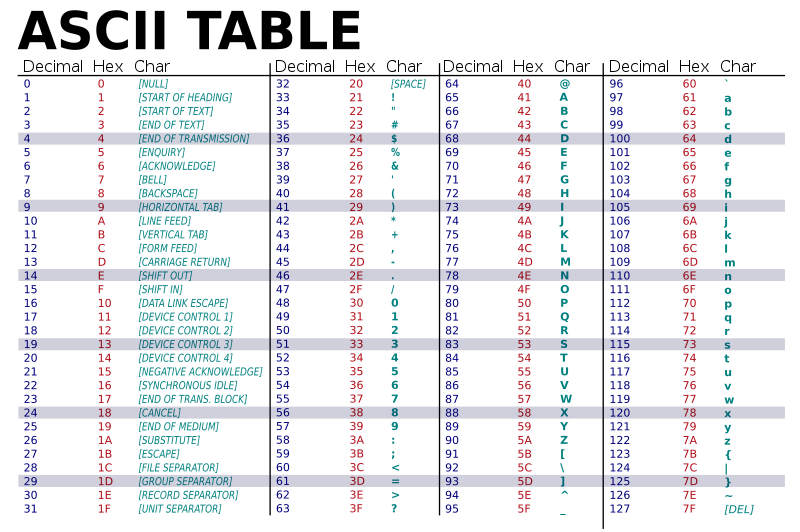
\includegraphics[scale=0.5]{ascii_table.png}
\end{figure}

\subsection{ASCII Table}
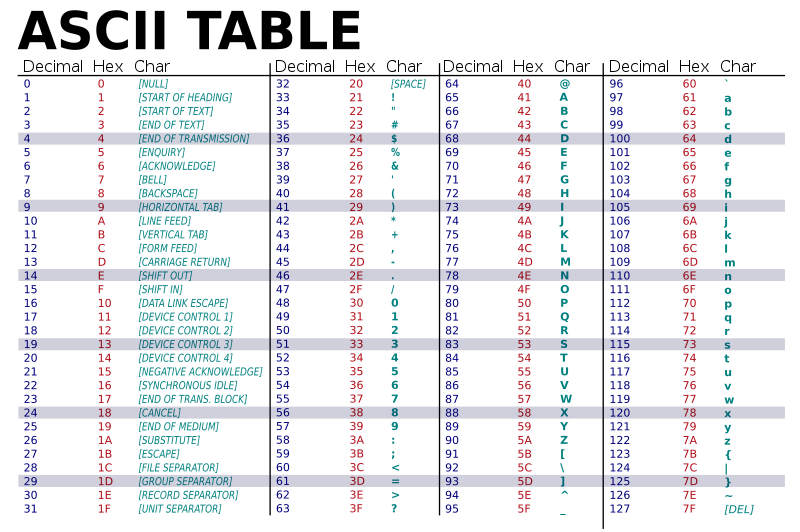
\includegraphics[scale=0.4]{ascii_table.png}
\subsection{One Second Time Complexity}
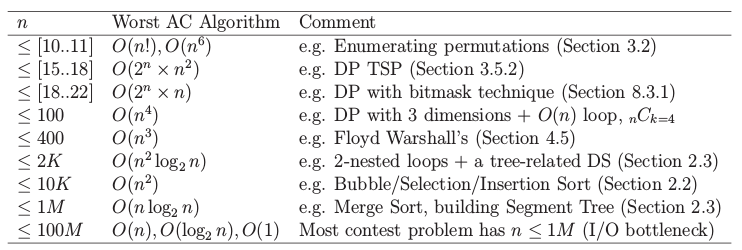
\includegraphics[scale=0.4]{one_second_time_complexity.png}

\subsection{Triângulo de Pascal}
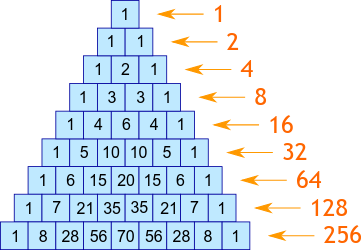
\includegraphics[scale=0.4]{pascal_triangle.png}

\subsection{Limite de Representação de Dados}
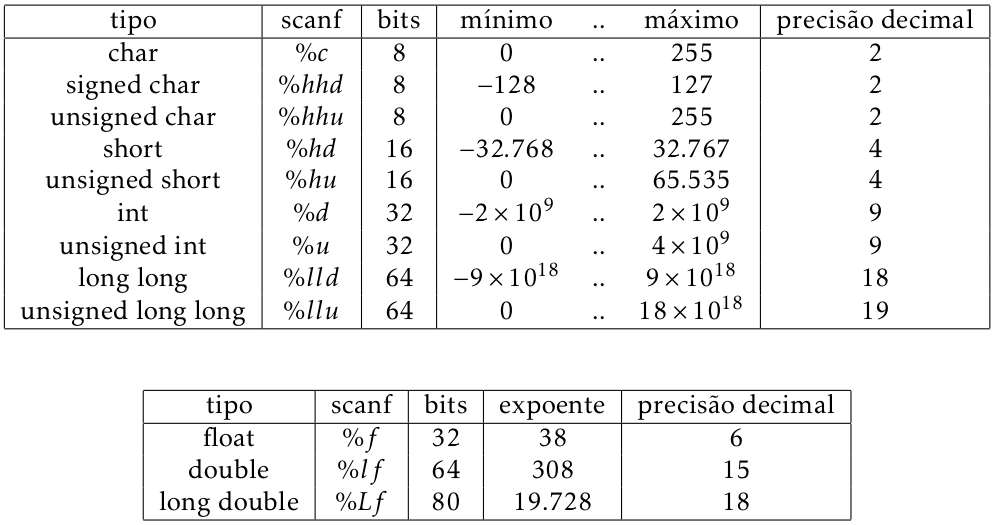
\includegraphics[scale=0.3]{limite_dados.png}

\subsection{Fatoriais}

Fatoriais até 20 com limites de tipo

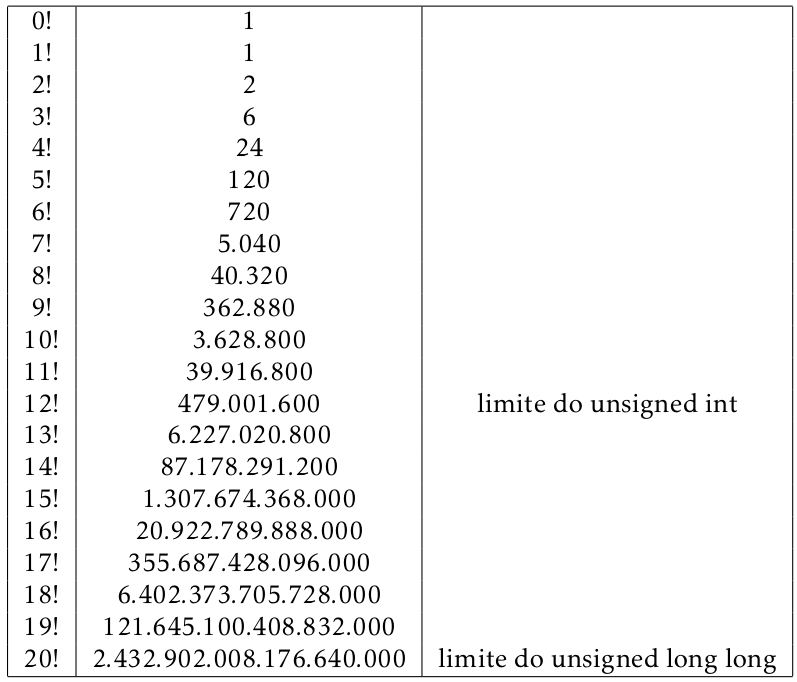
\includegraphics[scale=0.4]{fatorial.png}

\subsection{Quantidade de números primos de 1 até $10^n$}

É sempre verdade que n/ln(n) < pi(n) < 1.26 n/ln(n).

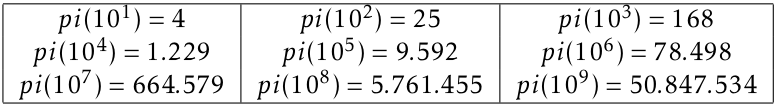
\includegraphics[scale=0.4]{quantidade_primos.png}

\subsection{Truques sujos (porém válidos)}
\begin{itemize}
   \item \textbf{Método Steve Halim:} As possíveis saídas do problema cabem no código do problema? Deixe um algoritmo naive
   brutando o problema na máquina por alguns minutos e escreva as respostas direto no código para submeter. Exemplo:
   problema cuja entrada é um único número da ordem de 105 . Verificar o tamanho máximo de caracteres de uma
   submissão
   \item \textbf{Problemas com constantes:} Se algum valor útil de algum problema for constante (independe da entrada), mas você
   não sabe, brute ele na sua máquina e cole no código
   \item \textbf{Debug com assert:} Pode colocar assert em código para submeter. Tente usar isso pra transformar um WA em um
   RTE. É uma forma válida de debug. Usar isso somente no desespero (fica gastando submissões)
\end{itemize}

\newpage